\documentclass{beamer}

% to include graphics
\usepackage{graphicx}

% to include hyperlinks
\usepackage{hyperref}

% divide slides into columns
\usepackage{multicol}


\usetheme{Copenhagen}
\usecolortheme{beaver}

\title{Cluster Progress}
\date{\today}

\begin{document}

%----------BEGIN TITLE----------

\begin{frame}
  \maketitle
\end{frame}

%-----------END TITLE-----------

%----------BEGIN NAS-0----------

\begin{frame}

  \frametitle{NAS-0 Resolution}

  \begin{itemize}
    \item New drive was automatically added to the incorrect unit by RAID card.
    \item Deleted incorrect unit.
    \item Started rebuild of RAID-1 array with newly unassigned drive.
  \end{itemize}

  \begin{figure}[H]
    \begin{center}
      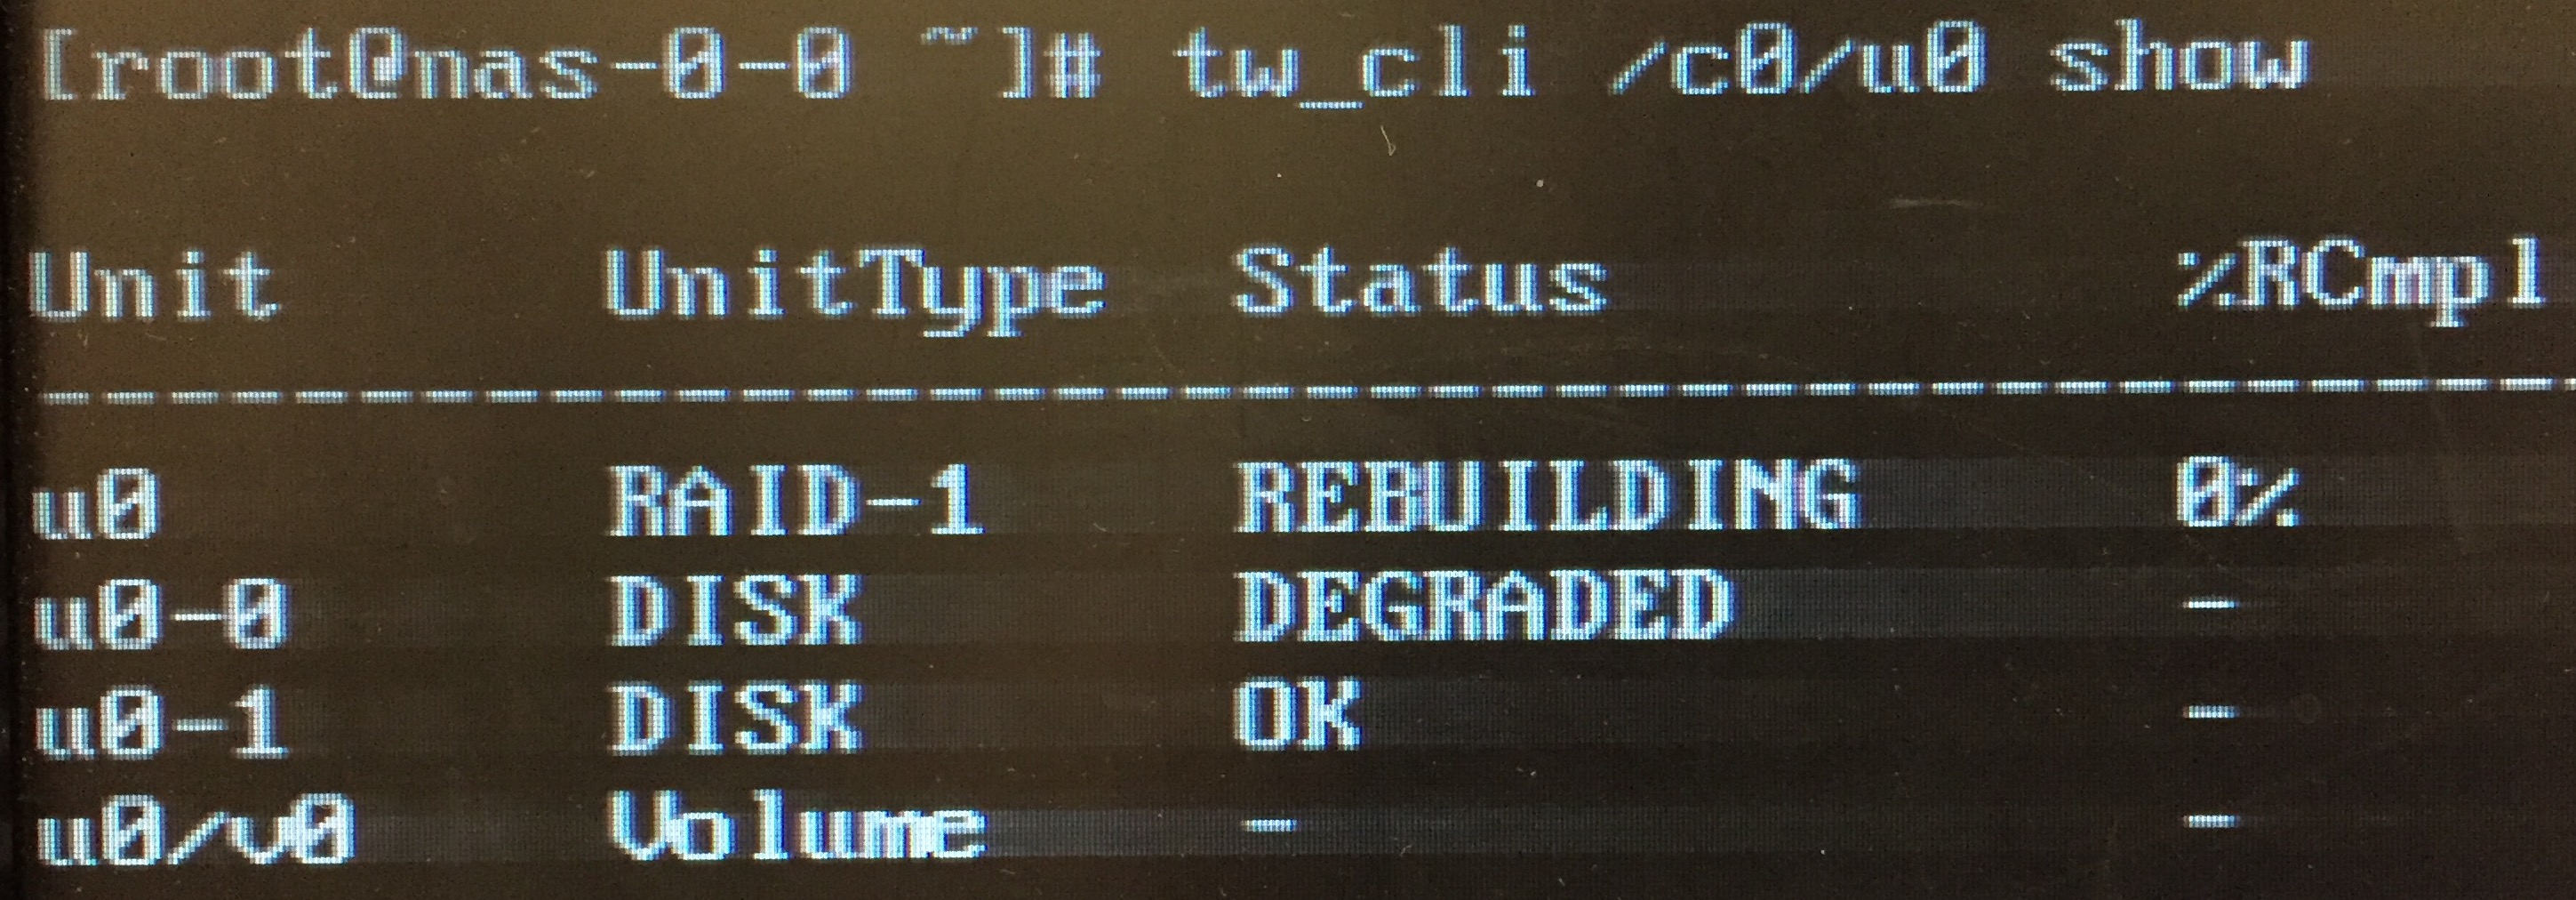
\includegraphics[width=0.7\textwidth]{nas0rebuild.jpg}
    \end{center}
    \caption{The output of {\tt tw\_cli /c0/u0 show rebuildstatus} on NAS-0.}
  \end{figure}

\end{frame}

%-----------END NAS-0-----------

%----------BEGIN OSG SOFTWARE SETUP----------

\begin{frame}

  \frametitle{Software Configuration}

  \begin{itemize}
    \item Tried to see if we could start bringing HTCondor online.
      \begin{itemize}
        \item HTCondor installed with OS; {\tt condor\_status} works out of the box
      \end{itemize}
    \item Host certificates needed for HTCondor configuration
    \item Hostcerts are typically requested in pairs; one for CE and one for SE
    \item Decided to begin configuration of SE first!
  \end{itemize}

  \begin{figure}[H]
    \begin{center}
      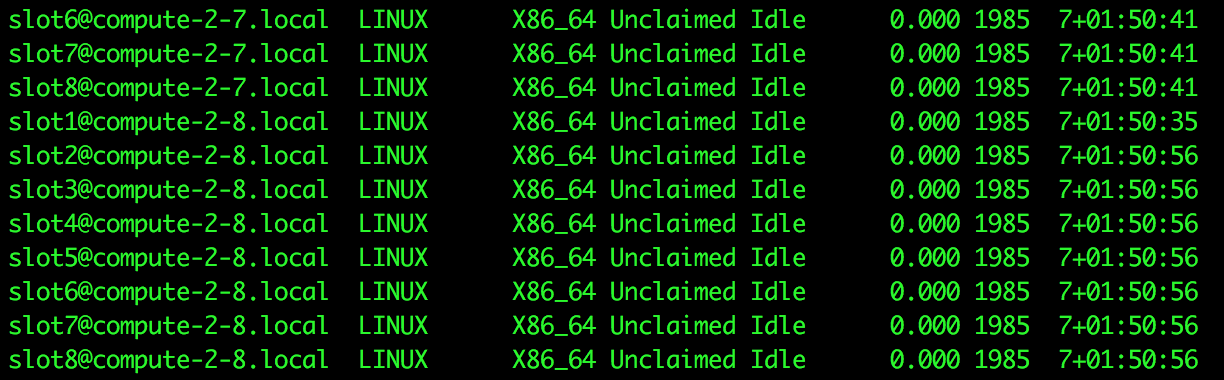
\includegraphics[width=0.7\textwidth]{condorStatus.png}
    \end{center}
    \caption{A snippet from the output of {\tt condor\_status} on the CE. It
      recognized all the available node CPUs.}
  \end{figure}

\end{frame}

%-----------END OSG SOFTWARE SETUP-----------

%----------BEGIN POSTER----------

\begin{frame}
  
  \frametitle{Senior Design Poster}

  \begin{center}
    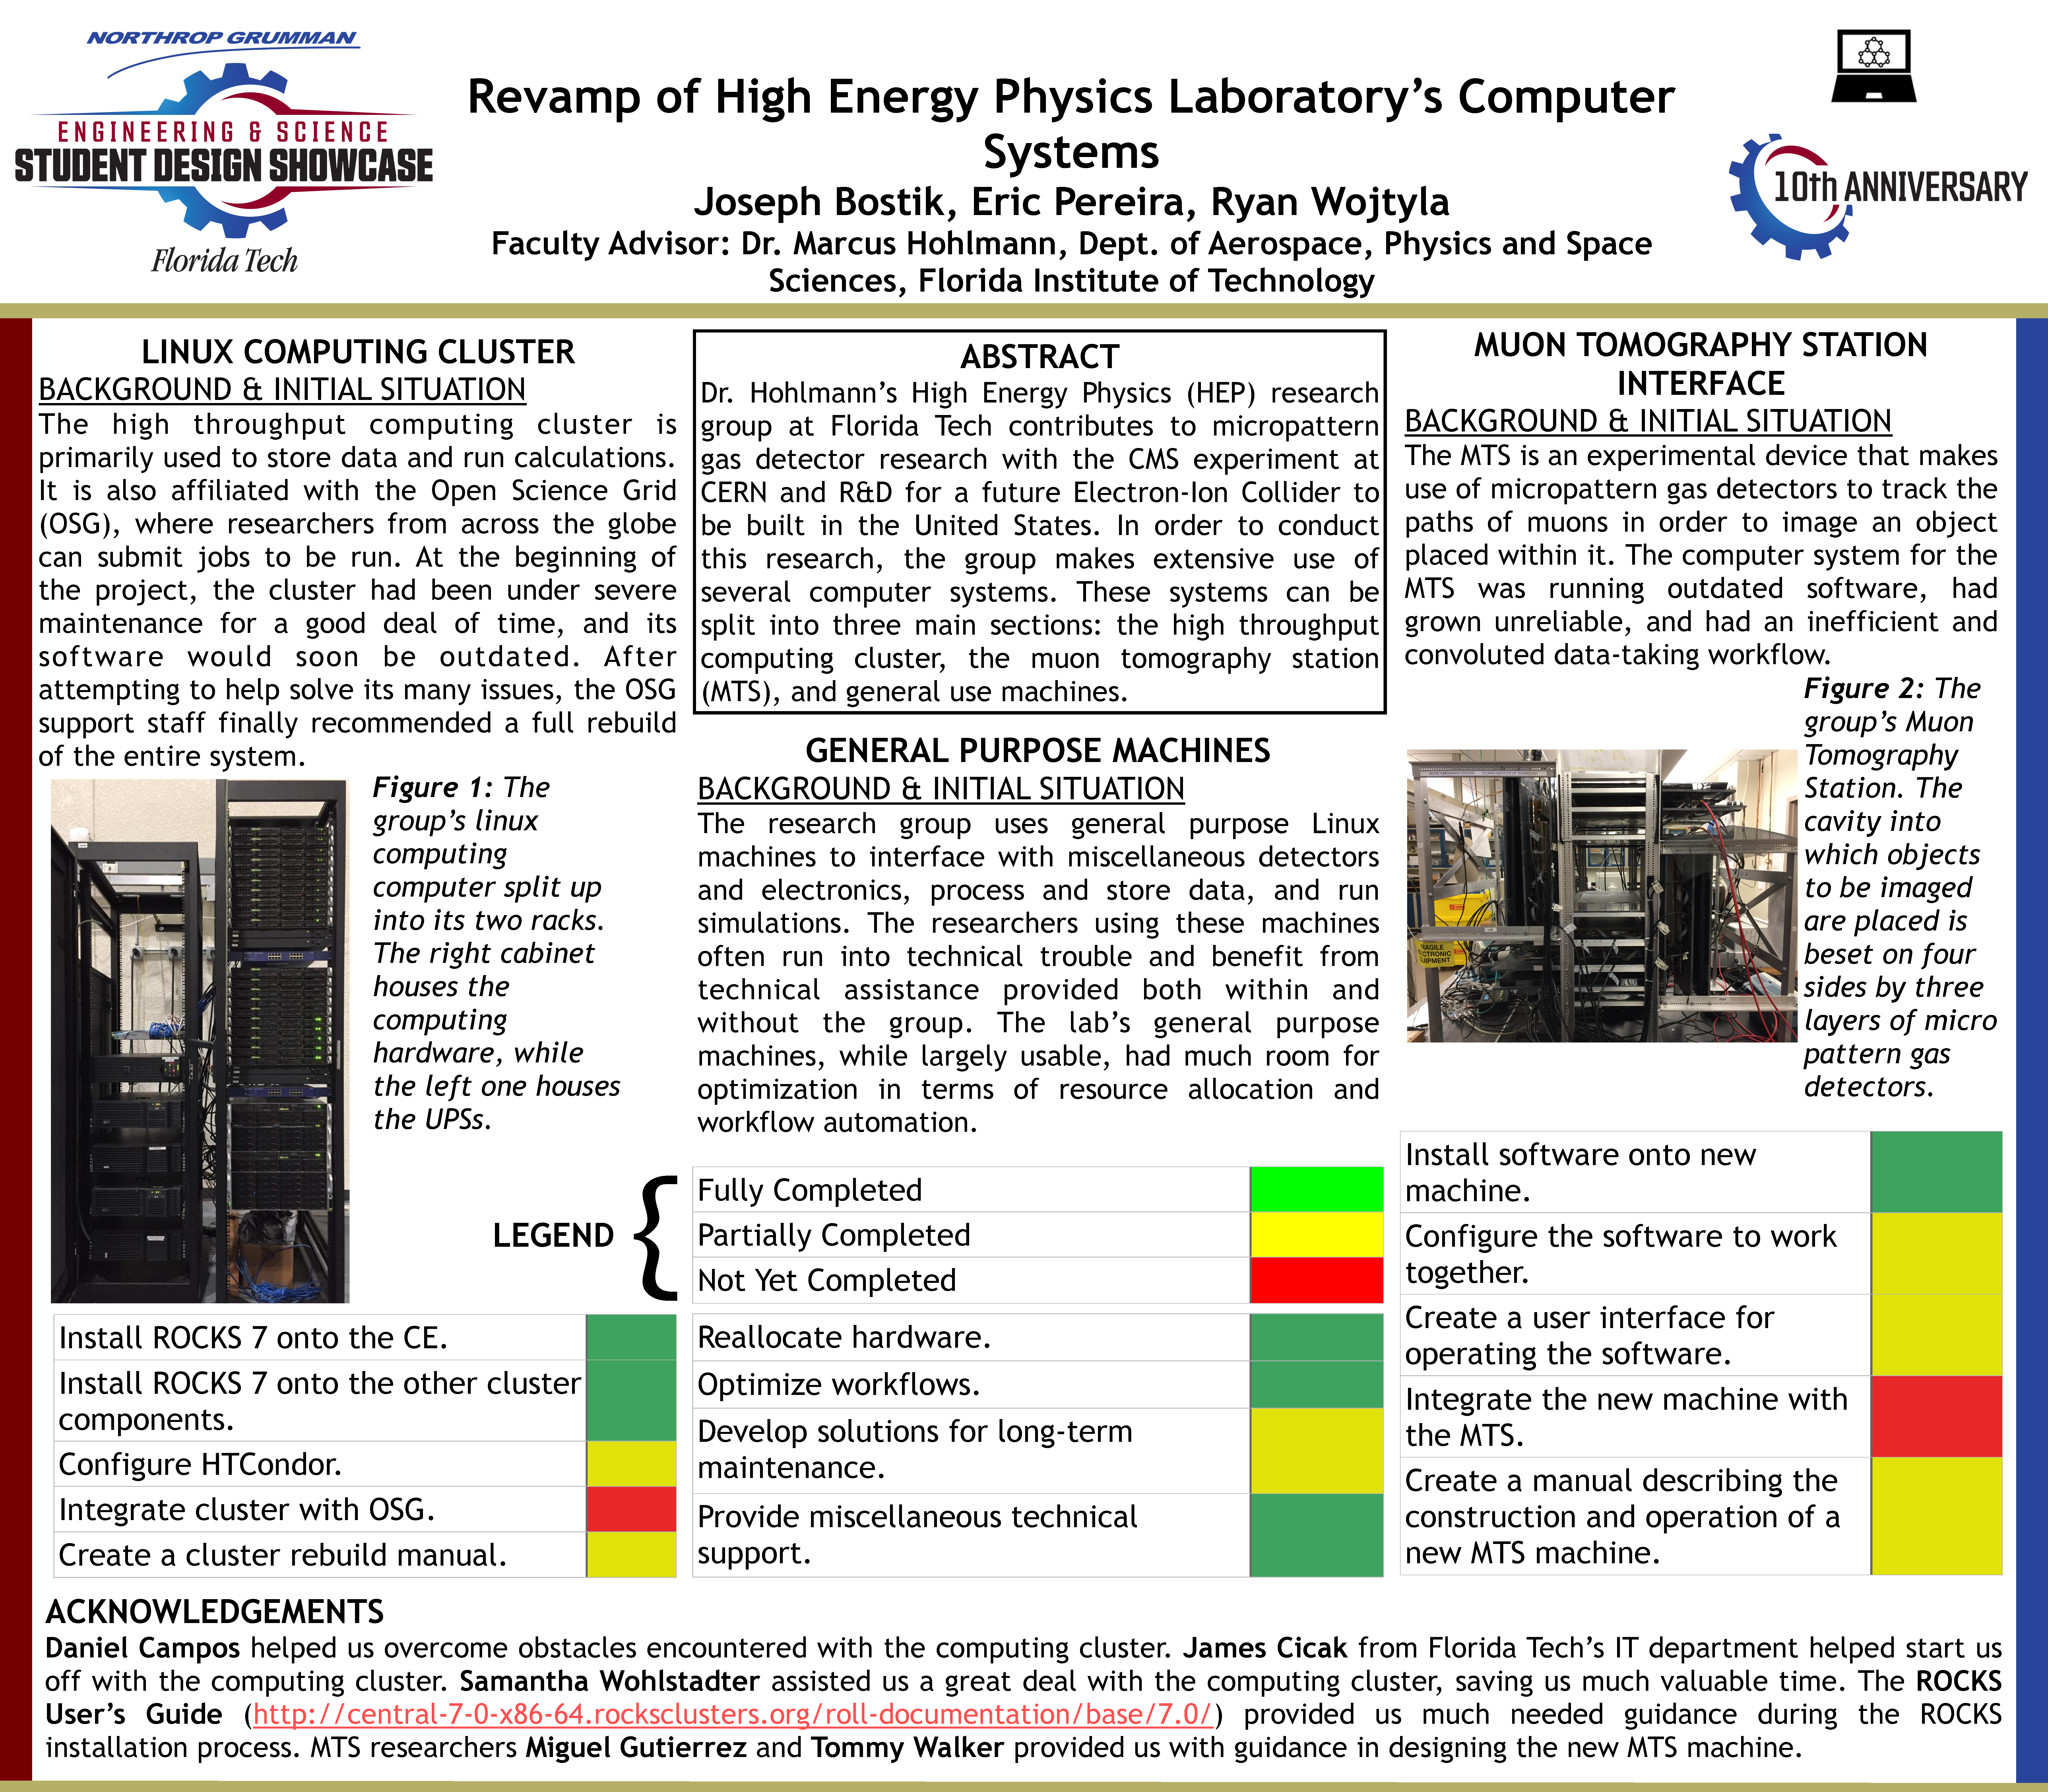
\includegraphics[width=0.8\textwidth]{poster.pdf}
  \end{center}

\end{frame}

%-----------END POSTER-----------



\end{document}

